\documentclass[14pt]{article}
\usepackage{graphicx} % Required for inserting images
\usepackage{float}
\usepackage{listings}
\usepackage[dvipsnames]{xcolor}
\usepackage{geometry}
\usepackage[UTF8]{ctex}
\usepackage{amsmath}
\usepackage{amsfonts}
\lstdefinestyle{python}{
  showstringspaces = false,
  frame=single,
  language=python,
  columns=fullflexible,
  basicstyle={\small\ttfamily},
  numbers=none,
  numberstyle=\tiny\color{blue},
  keywordstyle=\color{blue},
  commentstyle=\color{Bittersweet},
  stringstyle=\color{Bittersweet},
  breaklines=true,
  xleftmargin=0pt ,
  morekeywords={connect, read_sql_query,register,execute,fetchdf,cumsum,to_csv,close}
}

\title{Operations Research Homework 0}
\author{B10705034 資管三\ 許文鑫}
\geometry{a4paper,scale=0.8}
\begin{document}
\maketitle
\begin{enumerate}
    \item (30 points; 10 points each) Solve the following problems.
          \begin{enumerate}
              \item Let $f(x) = ax^2 +8x+6$, where $a \in \mathbb{R} $. Find all values of $a$ such that $f(x)$ is maximized at $x = 2$.\\
                    \textbf{Ans.}\\
                    If $f(x)$ is maximized at $x = 2$, then $f'(2) = 0$ and $f''(2) < 0$.\\
                    $f'(x) = 2ax+8, f''(x) = 2a$, so $f'(2) = 0 \Rightarrow 4a+8 = 0 \Rightarrow a = -2$,\\
                    $f''(2) = -4 < 0$.
              \item Let $f (x) = ax^2 + 8x + 6$, where $a \in \mathbb{R}$. Find $F(t) = \int^t_0f(x)dx$ as a function of $a$ and $t$ for all $t>0$.\\
                    \textbf{Ans. }
                    \begin{align*}
                        F(t) & = \int^t_0f(x)dx = \int^t_0(ax^2 + 8x + 6)dx  \\
                             & = \left.\frac{a}{3}x^3 + 4x^2 + 6x\right|^t_0 \\
                             & = \frac{a}{3}t^3 + 4t^2 + 6t
                    \end{align*}
              \item Find all values of $a \in R$ such that the inverse of
                    \[
                        \begin{bmatrix}
                            1 & 0 & 1 \\
                            a & 1 & 2 \\
                            3 & 1 & 4
                        \end{bmatrix}
                    \]
                    does not exist. If for all values of $a$ the inverse exists, prove it.\\
                    \textbf{Ans. }\\
                    The inverse of a matrix exists if and only if the determinant of the matrix is not zero.\\
                    The determinant of the matrix is
                    \begin{align*}
                        \begin{vmatrix}
                            1 & 0 & 1 \\
                            a & 1 & 2 \\
                            3 & 1 & 4
                        \end{vmatrix}
                         & =
                        1\begin{vmatrix}
                             1 & 2 \\
                             1 & 4
                         \end{vmatrix} -
                        0\begin{vmatrix}
                             a & 2 \\
                             3 & 4
                         \end{vmatrix} +
                        1\begin{vmatrix}
                             a & 1 \\
                             3 & 1
                         \end{vmatrix}               \\
                         & = 1(4-2) - 0(4-6) + 1(a-3) \\
                         & = 2 + a - 3                \\
                         & = a - 1
                    \end{align*}
                    The inverse of the matrix does not exist if and only if $a - 1 = 0 \Rightarrow a = 1$.
          \end{enumerate}
    \item (20 points; 10 points each) Consider the problem of determining whether a given integer $n$ is a prime number.
          \begin{enumerate}
              \item Write down a pseudocode of an algorithm that solves the problem for any given positive integer n. If you do not know what a pseudocode is, your may choose to write a real program in C++, Python, Java, or any modern language you like. Please indicate the language of your program. Still, as this term will show up again in this course, please teach yourself what a pseudocode is.\\
                    \textbf{Ans.}
                    \begin{lstlisting}[style=python]
bool is_prime(int n)
{
    int a = pow(n, 0.5);
    for (int i = 2; i <= a; i++)
    {
        if (n % i == 0)
        {
            return false;
        }
    }
    return true;
}
                    \end{lstlisting}
              \item What is the time complexity of your algorithm? Please use the big-O notation to express your solution.\\
                    \textbf{Ans.}\\
                    The time complexity of the algorithm is $O(\log n)$.
          \end{enumerate}
    \item (30 points; 10 points each) For each subproblem, use the graphical approach to solve
          \begin{align*}
              \text{max }  & 2x_1 +Ax_2              \\
              \text{s.t. } & x_1+x_2 \leq 8          \\
                           & 2x_1 - x_2 \geq 12      \\
                           & x_2 \leq B              \\
                           & x_1 \geq 0, x_2 \geq 0,
          \end{align*}
          for the given values of A and B. If there are multiple optimal solutions, please list just one of them. As long as there is at least one optimal solution, write one down and also list all constraints binding at that optimal solution. If there is no optimal solution, graphically demonstrate it.
          \begin{enumerate}
              \item $A=1,B=-4$.\\
                    \textbf{Ans. }
                    \begin{figure}[H]
                        \centering
                        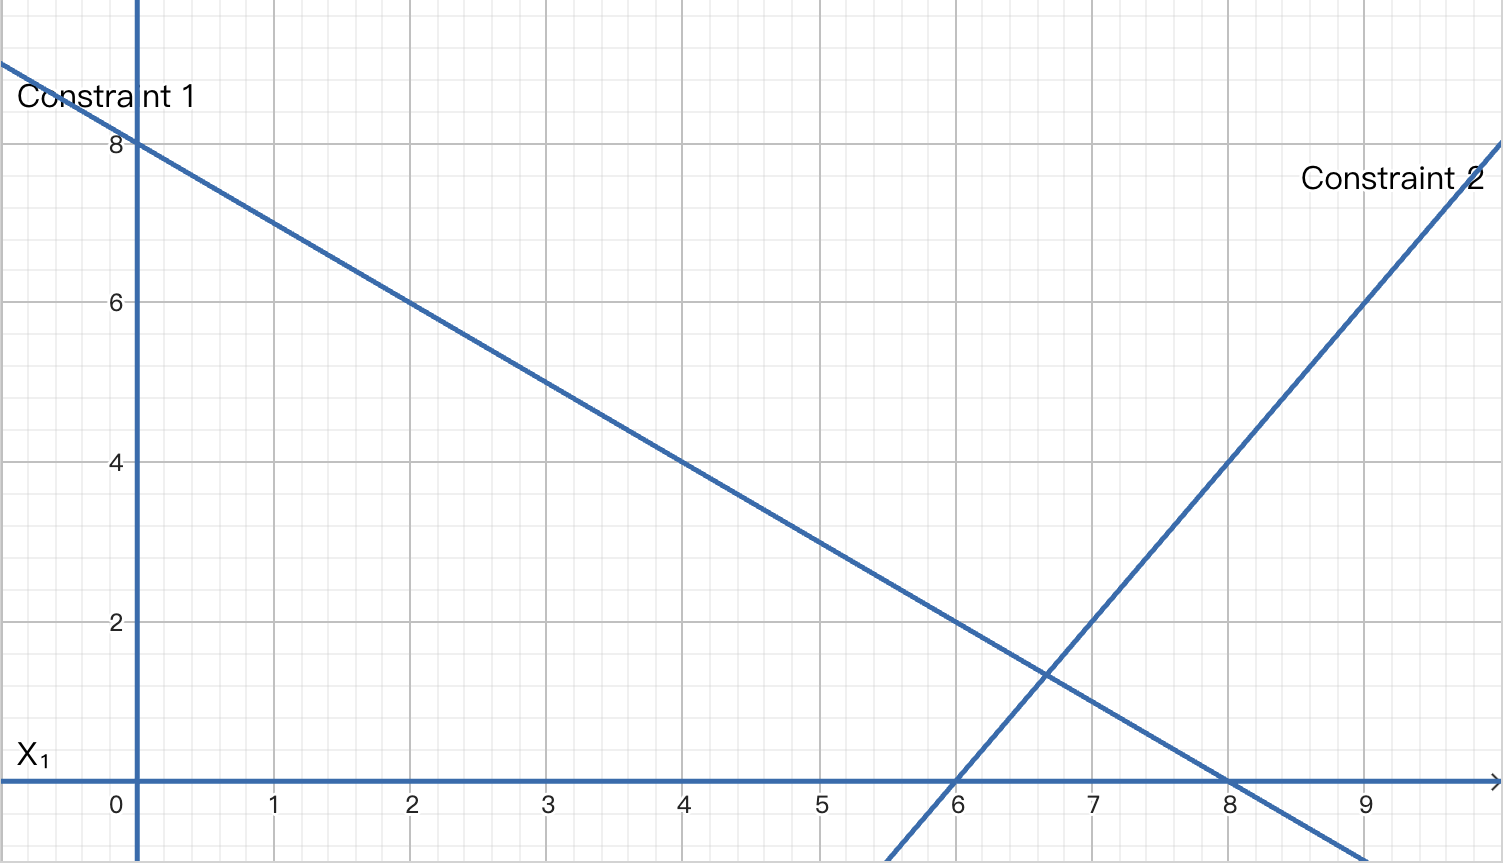
\includegraphics[width=0.5\textwidth]{p3_a.png}
                    \end{figure}
                    There's no optimal solution.
              \item $A=5, B =4$.\\
                    \textbf{Ans. }
                    \begin{figure}[H]
                        \centering
                        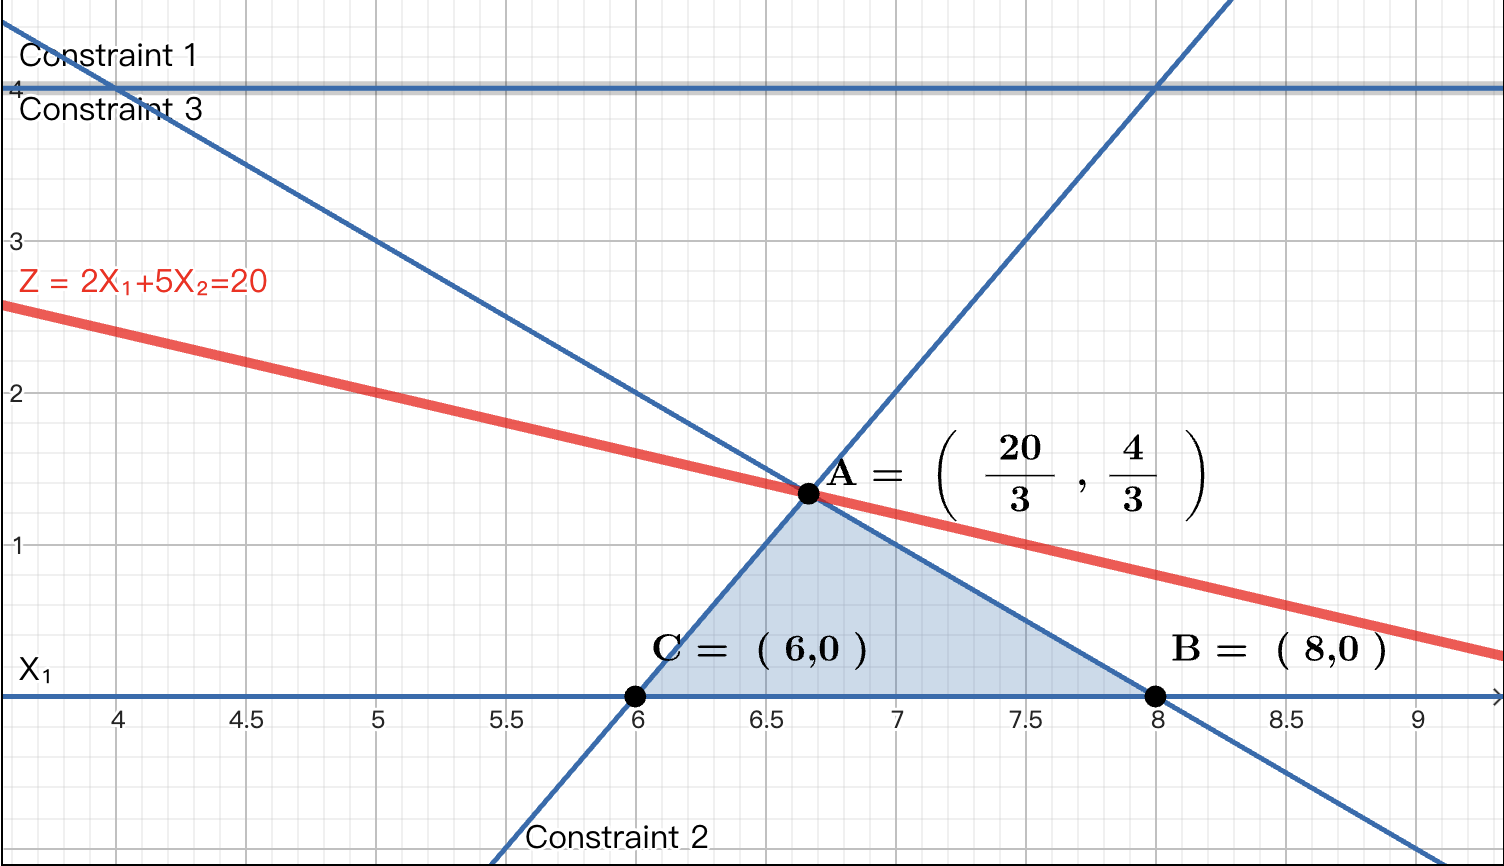
\includegraphics[width=0.5\textwidth]{p3_b.png}
                    \end{figure}
                    The optimal solution is $(\frac{20}{3},\frac{4}{3})$. The constraints binding at the optimal solution are $x_1+x_2 \leq 8$ and $2x_1 - x_2 \geq 12$.
              \item $A=-1,B=1$.\\
                    \textbf{Ans.}
                    \begin{figure}[H]
                        \centering
                        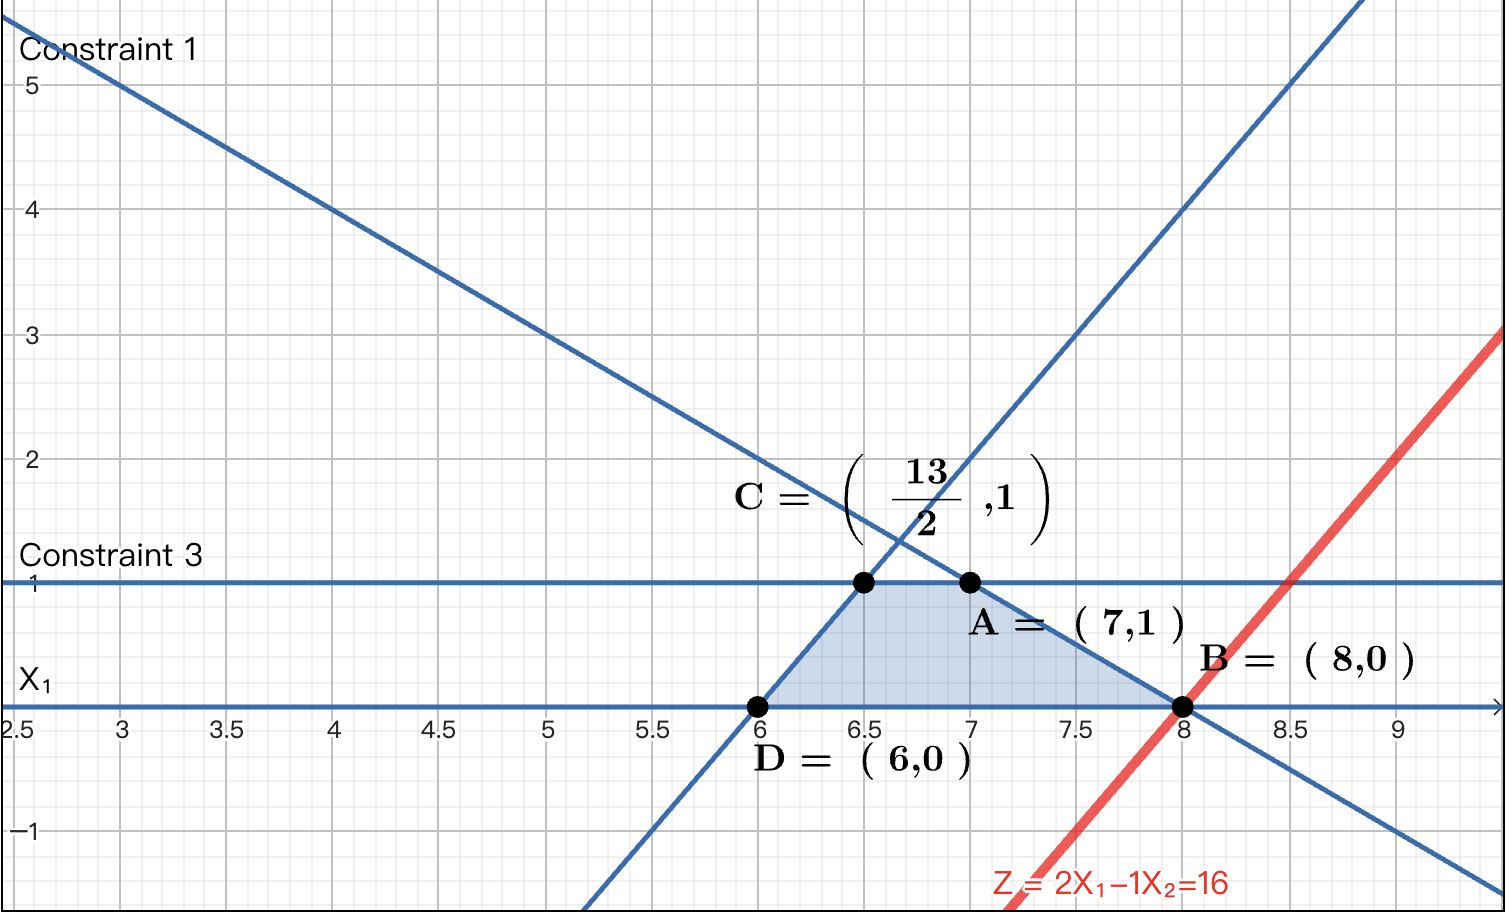
\includegraphics[width=0.5\textwidth]{p3_c.png}
                    \end{figure}
                    The optimal solution is $(8,0)$. The constraints binding at the optimal solution are $x_1+x_2 \leq 8$ and $x_1 \geq 0$.
          \end{enumerate}
    \item (20 points; 10 points each) For each of the following subproblems, formulate a linear program that maximizes IEDO’s profits for the next year.
          \begin{enumerate}
              \item IEDO Oil has refineries in Kaohsiung and Taipei. Currently, the Kaohsiung refinery can refine up to $K_1$ million barrels of oil per year, and the Taipei refinery up to $K_2$ million. Once refined, oil is shipped to two distribution points: Hsinchu and Taichung. IEDO Oil estimates that each distribution point can sell up to $D$ million barrels per year. Because of differences in shipping and refining costs, the profit earned per million barrels of oil shipped depends on where the oil was refined and on the point of distribution. In particular, the profit per million barrels is $P_{11}$ from Kaohsiung to Hsinchu, $P_{12}$ from Kaohsiung to Taichung, $P_{21}$ from Taipei to Hsinchu, and $P_{22}$ from Taipei to Taichung.\\
                    \textbf{Ans.}
                    \begin{table}[H]
                        \centering
                        \begin{tabular}{|c|c|c|}
                            \hline
                                      & Hsinchu  & Taichung \\
                            \hline
                            Kaohsiung & $P_{11}$ & $P_{12}$ \\
                            \hline
                            Taipei    & $P_{21}$ & $P_{22}$ \\
                            \hline
                        \end{tabular}
                    \end{table}
                    Let $x_{ij}$ be the number of million barrels of oil shipped from refinery $i$ to distribution point. The linear program is
                    \begin{align*}
                        \text{max }  & P_{11}x_{11} + P_{12}x_{12} + P_{21}x_{21} + P_{22}x_{22} \\
                        \text{s.t. } & x_{11} + x_{12} \leq K_1                                  \\
                                     & x_{21} + x_{22} \leq K_2                                  \\
                                     & x_{11} + x_{21} \leq D                                    \\
                                     & x_{12} + x_{22} \leq D                                    \\
                                     & x_{ij} \geq 0, \forall i = 1,2, \forall j = 1,2
                    \end{align*}
              \item IEDO Oil has refineries in $n$ cities. Currently, the refinery in city $i$ can refine up to $K_i$ million barrels of oil per year. Once refined, oil is shipped to $m$ distribution points. IEDO Oil estimates that each distribution point can sell up to $D$ million barrels per year. Because of differences in shipping and refining costs, the profit earned per million barrels of oil shipped depends on where the oil was refined and on the point of distribution. In particular, the profit per million barrels is $P_{ij}$ from refinery in city $i$ to distribution point $j$.\\
                    \textbf{Ans.}\\
                    Let $x_{ij}$ be the number of million barrels of oil shipped from refinery $i$ to distribution point. The linear program is
                    \begin{align*}
                        \text{max }  & \sum_{i=1}^n\sum_{j=1}^mP_{ij}x_{ij}                              \\
                        \text{s.t. } & \sum_{j=1}^mx_{ij} \leq K_i, \forall i = 1,2,...,n                \\
                                     & \sum_{i=1}^nx_{ij} \leq D , \forall j = 1,2,...,m                 \\
                                     & x_{ij} \geq 0, \forall i = 1,2,\cdots,n, \forall j = 1,2,\cdots,m
                    \end{align*}
          \end{enumerate}
\end{enumerate}
\end{document}